\thispagestyle{thachthuctoanhocnone}
\pagestyle{thachthuctoanhoc}
\everymath{\color{thachthuctoanhoc}}
\graphicspath{{../thachthuctoanhoc/pic/}}
\begingroup
\AddToShipoutPicture*{\put(0,616){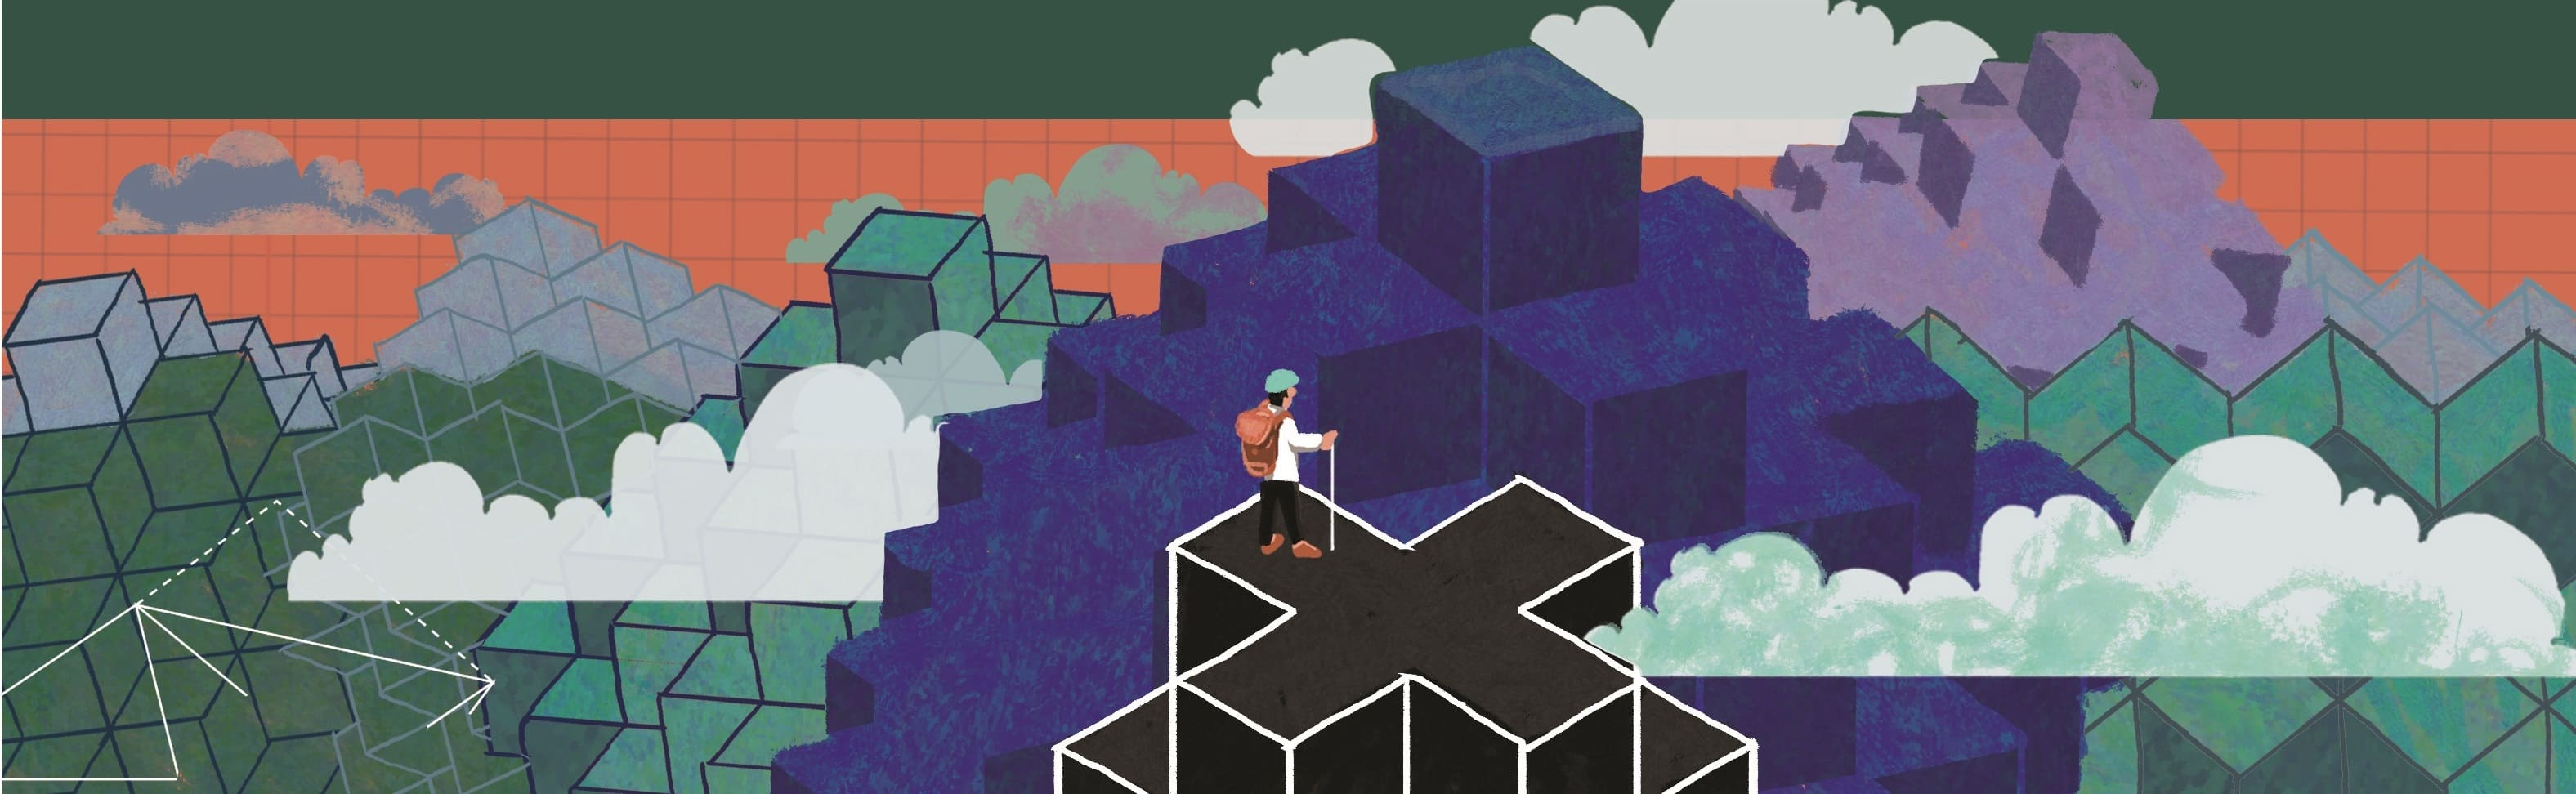
\includegraphics[width=19.3cm]{../thachthuctoanhoc/bannerthachthuc}}}
\centering
\vspace*{4cm}
\endgroup
\vspace*{-8pt}
\begin{tBox}
	\begin{itemize}[leftmargin = 13pt, itemsep = 1.0pt] 
		\item Mỗi bài toán đề xuất (kèm theo lời giải) cần được nêu rõ là bài sáng tác hay bài sưu tầm.
		%		\item Mỗi bài toán đề xuất (kèm theo lời giải) cần được nêu rõ là bài sáng tác hay bài sưu tầm (nếu là bài sưu tầm, cần ghi rõ nguồn).
		\item Bài giải cho mỗi bài toán cần được trình bày trong một file riêng hoặc
		một tờ giấy riêng.
		\item  Người đề xuất bài toán hoặc gửi bài giải cho các bài toán trong mục ``Thách thức kỳ này" cần ghi rõ họ, đệm, tên và nơi làm việc/học tập, số điện thoại liên hệ. Nếu là học sinh (hoặc sinh viên) cần ghi rõ là học sinh lớp mấy (hoặc sinh viên năm thứ mấy).
		\item Các bài toán trong mục Thách thức kỳ này hướng tới các độc giả là học sinh phổ thông; được phân chia thành các mức độ $B$, $A$, và được sắp xếp theo độ khó tăng dần, theo đánh giá chủ quan của Ban biên tập. Các bài toán mức độ $B$ không đòi hỏi các kiến thức vượt quá chương trình môn Toán cấp THCS; các bài toán mức độ $A$ không đòi hỏi các kiến thức vượt quá chương trình môn Toán cấp THPT.
		\item Cách thức gửi bài toán đề xuất hoặc lời giải: gửi file thu được bằng cách scan, ảnh chụp (rõ nét) của bản viết tay, hoặc được soạn thảo bằng các phần mềm Latex, Word tới \url{bbt@pi.edu.vn} hoặc gửi qua đường bưu điện tới Tòa soạn (xem địa chỉ tại bìa $2$).
		\item Hạn gửi lời giải cho các bài toán P$651$--P$660$: trước ngày $15/1/2023$.
	\end{itemize}
\end{tBox}
\begin{center}
	\vspace*{-5pt}
	\textbf{\color{thachthuctoanhoc}\color{thachthuctoanhoc}\color{thachthuctoanhoc}THÁCH THỨC KỲ NÀY}
	\vspace*{-5pt}
\end{center}
\begin{multicols}{2}
	\setlength{\abovedisplayskip}{4pt}
	\setlength{\belowdisplayskip}{4pt}
	{\color{thachthuctoanhoc}{\usefont{T5}{qag}{b}{n} P661.}}
	(Mức $B$) Một xấp tiền giấy có $120$ tờ tiền, gồm các tờ tiền với mệnh giá $10.000$ đồng, $50.000$ đồng, và $100.000$ đồng. Số tờ tiền mệnh giá $50.000$ đồng là một số lớn hơn $5$ và chia hết cho $5$. Hỏi mỗi loại mệnh giá có bao nhiêu tờ tiền? Biết rằng, tổng mệnh giá của cả xấp tiền là $8.600.000$ đồng.
	\begin{flushright}
		\textit{Đăng Hải, Hà Nội}
	\end{flushright}
	{\color{thachthuctoanhoc}{\usefont{T5}{qag}{b}{n} P662.}}
	(Mức $B$) Với mỗi số thực $x$, đặt $f(x)=\sqrt[3]{x^3-x}$. Cho các số thực đôi một phân biệt $a,b,c$ thoả mãn
	\begin{align*}
		&a f(b)+b f(c)+c f(a)\\
		=\,&a f(c)+b f(a)+c f(b)=0.
	\end{align*}
	Chứng minh rằng $a+b+c=0$. 
	\begin{flushright}
		\textit{Phan Quang Đạt, Hà Nội}
	\end{flushright}
	{\color{thachthuctoanhoc}{\usefont{T5}{qag}{b}{n} P663.}}
	(Mức $B$) Cho hai đường tròn đồng tâm $(C_1)$ và $(C_2)$, có bán kính, tương ứng, là $14$ và $50$. Tìm số nguyên dương $k$ nhỏ nhất có tính chất: Nếu qua một điểm tuỳ ý nằm trên $(C_1)$, kẻ $k$ dây cung tuỳ ý của $(C_2)$ thì chắc chắn có một dây cung có độ dài không nguyên. 
	\vskip 0.05cm
	\hfill	\textit{Hà Duy Hưng, Hà Nội}
	\vskip 0.05cm
	{\color{thachthuctoanhoc}{\usefont{T5}{qag}{b}{n} P664.}}
	(Mức $B$) Giải hệ phương trình
	\begin{align*}
		\begin{cases}
			x^{23}=3y^{21}-2z^{19}&\\
			y^{23}=3z^{21}-2x^{19}&\\
			z^{23}=3x^{21}-2y^{19}.
		\end{cases}
	\end{align*}
	\hfill	\textit{Bằng Linh, Phú Thọ}
	\vskip 0.05cm
	{\color{thachthuctoanhoc}{\usefont{T5}{qag}{b}{n} P665.}}
	(Mức $B$) Cho số thực $k\ge1$, và cho tam giác đều $ABC$ cạnh $a$. Một điểm $M$ di động trên đường tròn ngoại tiếp của tam giác đó. Hãy tìm giá trị nhỏ nhất và lớn nhất của biểu thức $S=kMA+MB+MC$.
	\begin{figure}[H]
		\vspace*{-10pt}
		\centering
		\captionsetup{labelformat= empty, justification=centering}
		\definecolor{ffqqqq}{rgb}{1,0,0}
		\definecolor{qqzzcc}{rgb}{0,0.6,0.8}
		\definecolor{qqqqff}{rgb}{0,0,1}
		\definecolor{qqqqffa}{rgb}{1,1,1}
		\definecolor{cqcqcq}{rgb}{0.7529411764705882,0.7529411764705882,0.7529411764705882}
		\begin{tikzpicture}[scale=0.6,node font = \small]
			\draw [color=qqzzcc] (0,3.196152422706632)-- (-3,-2);
			\draw [color=qqzzcc] (-3,-2)-- (3,-2);
			\draw [color=qqzzcc] (3,-2)-- (0,3.196152422706632);
			\draw [,color=ffqqqq] (0,-0.2679491924311226) circle (3.4641016151377544cm);
			\draw [] (1.473281922635266,-3.4031430263808087)-- (3,-2);
			\draw [] (-3,-2)-- (1.473281922635266,-3.4031430263808087);
			\draw [] (1.473281922635266,-3.4031430263808087)-- (0,3.196152422706632);
			\draw [fill=qqqqffa] (-3,-2) circle (1.6pt);
			\draw[color=qqqqff] (-3.38,-2.35) node {$B$};
			\draw [fill=qqqqffa] (3,-2) circle (1.6pt);
			\draw[color=qqqqff] (3.34,-2.27) node {$C$};
			\draw [fill=qqqqffa] (0,3.196152422706632) circle (1.6pt);
			\draw[color=qqqqff] (0,3.75) node {$A$};
			\draw [fill=qqqqffa] (1.473281922635266,-3.4031430263808087) circle (1.6pt);
			\draw[color=qqqqff] (1.65,-3.75) node {$M$};
			\draw [fill=qqqqffa] (0,-0.2679491924311226) circle (1.6pt);
			\draw[color=qqqqff] (-0.4,-0.13) node {$O$};
		\end{tikzpicture}
		\vspace*{-10pt}
	\end{figure}
	\hfill	\textit{Hoàng Ngọc Minh, Hà Nội}
	\vskip 0.1cm
	{\color{thachthuctoanhoc}{\usefont{T5}{qag}{b}{n} P666.}}
	(Mức $B$) Cho số nguyên $n\ge13$. Chứng minh rằng, không thể chia một hình vuông cạnh $n$ thành năm hình chữ nhật, với độ dài các cạnh là $1,2,3,4,5,6,7,8,9,10$, như hình dưới đây.
	\begin{figure}[H]
		\vspace*{-10pt}
		\centering
		\captionsetup{labelformat= empty, justification=centering}
		\definecolor{qqqqff}{rgb}{0,0,1}
		\definecolor{qqqqffa}{rgb}{1,1,1}
		\begin{tikzpicture}[thachthuctoanhoc,scale=0.35]
			\draw [] (-5,5)-- (5,5);
			\draw [] (5,5)-- (5,-5);
			\draw [] (-5,5)-- (-5,-5);
			\draw [] (-5,-5)-- (5,-5);
			\draw [] (-1.8064850795005638,5)-- (-1.806485079500564,-0.9133587450621485);
			\draw [] (-5,-0.9133587450621485)-- (1.4776647785694939,-0.9133587450621485);
			\draw [] (1.4776647785694939,1.1789625354824862)-- (1.477664778569494,-5);
			\draw [] (-1.806485079500564,1.1789625354824862)-- (5,1.1789625354824862);
			\draw [fill=qqqqffa] (-5,5) circle (1.6pt);
			\draw [fill=qqqqffa] (5,5) circle (1.6pt);
			\draw [fill=qqqqffa] (5,-5) circle (1.6pt);
			\draw [fill=qqqqffa] (-5,-5) circle (1.6pt);
			\draw [fill=qqqqffa] (-1.8064850795005638,5) circle (1.6pt);
			\draw [fill=qqqqffa] (5,1.1789625354824862) circle (1.6pt);
			\draw [fill=qqqqffa] (-5,-0.9133587450621485) circle (1.6pt);
			\draw [fill=qqqqffa] (1.477664778569494,-5) circle (1.6pt);
			\draw [fill=qqqqffa] (-1.806485079500564,1.1789625354824862) circle (1.6pt);
			\draw [fill=qqqqffa] (1.4776647785694939,1.1789625354824862) circle (1.6pt);
			\draw [fill=qqqqffa] (1.4776647785694939,-0.9133587450621485) circle (1.6pt);
			\draw [fill=qqqqffa] (-1.806485079500564,-0.9133587450621485) circle (1.6pt);
		\end{tikzpicture}
		\vspace*{-10pt}
	\end{figure}
	\hfill\textit{Phạm Như Ngọc, Hải Phòng}
	\vskip 0.1cm
	{\color{thachthuctoanhoc}{\usefont{T5}{qag}{b}{n} P667.}}
	(Mức $A$) Chứng minh rằng
	\begin{align*}
		8(x+y-1)^2-9xy(x+y-1)+xy\ge0
	\end{align*}
	với mọi $x,y\in[0;1]$. 
	\vskip 0.1cm
		\hfill\textit{Nguyễn Tấn Mạnh và Nguyễn Anh Vũ}, 
		\vskip 0.01cm
		\hfill \textit{Bình Định}
	\vskip 0.1cm
	{\color{thachthuctoanhoc}{\usefont{T5}{qag}{b}{n} P668.}}
	(Mức $A$) Cho số nguyên $n\ge2$. Có $n$ con ếch nằm trên một trục số, tại $n$ điểm tuỳ ý, thuộc tập $2n$ điểm $1,2,\ldots,2n$. Vào cùng một thời điểm, mỗi con ếch đều nhảy đến một trong số $n$ điểm còn lại, thuộc tập $2n$ điểm vừa nêu, sao cho không có hai con nào cùng nhảy tới một điểm. Chứng minh rằng
	\vskip 0.05cm
	$a)$ Tổng khoảng cách $n$ con ếch đã nhảy không vượt quá $n^2$. 
	\vskip 0.05cm
	$b)$ Tồn tại một phương án nhảy của $n$ con ếch, sao cho tổng khoảng cách chúng đã nhảy đúng bằng $n^2$. 
	\vskip 0.1cm
	\hfill	\textit{Lê Vĩ, Hà Nội}
	\vskip 0.1cm
	{\color{thachthuctoanhoc}{\usefont{T5}{qag}{b}{n} P669.}}
	(Mức $A$) Cho tam giác nhọn $ABC$, với $AB<AC$, nội tiếp đường tròn $(O)$. Gọi $M,N$ tương ứng là trung điểm của các cung $BC$ lớn và cung $BC$ nhỏ. Trên đường thẳng $AN$, lấy điểm $D$ sao cho $D$ nằm trong tam giác $ABC$ và không trùng với tâm đường tròn nội tiếp tam giác ấy. Trên đoạn thẳng $MD$, lấy điểm $T$ sao cho $\angle{MBT}=\angle{DCB}$. Chứng minh rằng trực tâm của tam giác $TND$ nằm trên đường thẳng $BC$.
	\begin{figure}[H]
		\vspace*{-10pt}
		\centering
		\captionsetup{labelformat= empty, justification=centering}
		\definecolor{qqwuqq}{rgb}{0,0.39215686274509803,0}
		\definecolor{ffqqqq}{rgb}{1,0,0}
		\definecolor{qqzzff}{rgb}{0,0.6,1}
		\definecolor{qqqqff}{rgb}{0,0,1}
		\definecolor{qqqqffa}{rgb}{1,1,1}
		\begin{tikzpicture}[scale=0.5,node font = \small]
			\draw [shift={(-4.52,-2)},color=qqwuqq] (0,0) -- (44.80816980779454:0.9) arc (44.80816980779454:59.48716265964927:0.9) -- cycle;
			\draw [shift={(3,-2)},,color=qqwuqq] (0,0) -- (165.3210071481453:0.9) arc (165.3210071481453:180:0.9) -- cycle;
			\draw [color=qqzzff] (-3.08,3.7)-- (-4.52,-2);
			\draw [color=qqzzff] (-4.52,-2)-- (3,-2);
			\draw [color=qqzzff] (3,-2)-- (-3.08,3.7);
			\draw [color=ffqqqq] (-0.76,0.082) circle (4.297944159711711cm);
			\draw [] (-3.08,3.7)-- (-0.76,-4.215944159711711);
			\draw [] (-1.7761254755175533,-0.7488784168421159)-- (3,-2);
			\draw [] (-4.52,-2)-- (-0.76,4.379944159711711);
			\draw [] (-4.52,-2)-- (-1.4124345691125013,1.0868261064673503);
			\draw [] (-1.7761254755175533,-0.7488784168421159)-- (-0.76,4.379944159711711);
			\draw [] (-1.4124345691125013,1.0868261064673503)-- (-0.76,-4.215944159711711);
			\draw [shift={(-4.52,-2)},,color=qqwuqq] (44.80816980779454:0.9) arc (44.80816980779454:59.48716265964927:0.9);
			\draw[,color=qqwuqq] (-4.0045520409083055,-1.3367403212404605) -- (-3.9309166181809205,-1.241988938560526);
			\draw [shift={(3,-2)},,color=qqwuqq] (165.3210071481453:0.9) arc (165.3210071481453:180:0.9);
			\draw[,color=qqwuqq] (2.1668824426700812,-1.8926913998384574) -- (2.0478656487658085,-1.8773615998153805);
			\draw [fill=qqqqffa] (-3.08,3.7) circle (1.6pt);
			\draw[color=qqqqff] (-3.2,4.19) node {$A$};
			\draw [fill=qqqqffa] (-4.52,-2) circle (1.6pt);
			\draw[color=qqqqff] (-4.99,-2.19) node {$B$};
			\draw [fill=qqqqffa] (3,-2) circle (1.6pt);
			\draw[color=qqqqff] (3.44,-2.29) node {$C$};
			\draw [fill=qqqqffa] (-0.76,4.379944159711711) circle (1.6pt);
			\draw[color=qqqqff] (-0.82,4.81) node {$M$};
			\draw [fill=qqqqffa] (-0.76,-4.215944159711711) circle (1.6pt);
			\draw[color=qqqqff] (-0.8,-4.7) node {$N$};
			\draw [fill=qqqqffa] (-1.7761254755175533,-0.7488784168421159) circle (1.6pt);
			\draw[color=qqqqff] (-2.2,-0.95) node {$D$};
			\draw [fill=qqqqffa] (-1.4124345691125013,1.0868261064673503) circle (1.6pt);
			\draw[color=qqqqff] (-1,1.1) node {$T$};
		\end{tikzpicture}
		\vspace*{-10pt}
	\end{figure}
	\hfill\textit{Đỗ Đại Phong, Thừa Thiên Huế}
	\vskip 0.1cm
	{\color{thachthuctoanhoc}{\usefont{T5}{qag}{b}{n} P670.}}
	(Mức $A$) Hỏi, có thể chọn được tối đa bao nhiêu điểm nguyên trong mặt phẳng toạ độ, sao cho đoạn thẳng nối hai điểm bất kỳ trong chúng chứa đúng $2022$ điểm nguyên?
	\vskip 0.05cm
	(Trong mặt phẳng toạ độ, một điểm được gọi là {\it điểm nguyên}, nếu cả hoành độ và tung độ của nó đều là các số nguyên.)
	\vskip 0.1cm
	\hfill	\textit{Nguyễn Thành Khang, Hà Nội}
\end{multicols}
\centerline{{\large{\textbf{\color{thachthuctoanhoc}GIẢI BÀI KỲ TRƯỚC}}}}
\vspace*{-5pt}
\begin{multicols}{2}
	\setlength{\abovedisplayskip}{4pt}
	\setlength{\belowdisplayskip}{4pt}
	{\color{thachthuctoanhoc}{\usefont{T5}{qag}{b}{n} P641.}}
	(Mức $B$)
	Tại mỗi đỉnh của một đa giác lồi $18$ cạnh ở hình dưới đây, người ta ghi một số, sao cho số được ghi ở mỗi đỉnh bằng tổng hai số được ghi ở hai đỉnh kề với nó.
	
	%Hình vẽ
	
	Biết rằng, số được ghi ở đỉnh $X$ là $20$, và số được ghi ở đỉnh $Y$ là $22$. Hãy tìm số được ghi ở đỉnh $S$.
	\vskip 0.05cm
	\textbf{Lời giải} (\textit{phỏng theo ý giải của bạn Nguyễn Chánh Thiện, lớp $8/14$, trường THCS Lê Quý Đôn, Quận $3$, Tp. Hồ Chí Minh})\textbf{.}
	\vskip 0.05cm
	Xuất phát từ đỉnh $S$, theo chiều kim đồng hồ, kí hiệu các số được ghi tại các đỉnh của $18$--giác, lần lượt, bởi  $x_1,  x_2, \ldots, x_{18}$ (xem Hình dưới đây).
	
	%%%
	Do $x_8$, $x_{12}$ là các số được ghi tại các đỉnh $X$, $Y$, nên theo giả thiết của bài ra, $x_8 =20$  và  $x_{12} = 22$.
	\vskip 0.05cm
	Từ qui tắc ghi số của đề bài suy ra, với mỗi $k = 1, 2, \ldots, 15$, ta có:
	\begin{align*}
		{x_k}\, = \,\,{x_{k\,\, + \,\,1}}\, - \,\,{x_{k\,\, + \,\,2}}\, = \,\,{x_{k\,\, + \,\,1}}\, - \,\,\left( {{x_{k\,\, + \,\,1}}\, + \,\,{x_{k\,\, + \,\,3}}} \right)\, = \,\, - {x_{k\,\, + \,\,3}}.
	\end{align*}
	Do đó
		\begin{align*}
			&{x_2}\, = \,\, - {x_5}\, = \,\,{x_8}\, = \,\,20,\\
			&22\,\, = \,\,{x_{12}}\, = \,\, - {x_{15}}\, = \,\,{x_{18}}.7
		\end{align*}
	Vì vậy
	\begin{align*}
		{x_1}\, = \,\,{x_{18}}\, + \,\,{x_2}\, = \,\,22\,\, + \,\,20\,\, = \,\,42.
	\end{align*}
	Vậy, số được ghi ở đỉnh $S$ là $42$.
	\vskip 0.05cm
	\textbf{Bình luận và Nhận xét}
	\vskip 0.05cm	
	Tạp chí đã nhận được nhiều lời giải cho bài toán, từ bạn đọc; và tất cả những lời giải này đều là lời giải đúng.
	\begin{flushright}
		\textbf{Lê Huy}
	\end{flushright}
	{\color{thachthuctoanhoc}{\usefont{T5}{qag}{b}{n} P641.}}
	(Mức $B$)
	Cho $x$, $y$ là các số nguyên dương thỏa mãn $y^2 + x - 1$ chia hết cho $xy + 1$. Chứng minh rằng, tồn tại số tự nhiên $z$, sao cho $x + y + z + xyz$ là một số chính phương.
	\vskip 0.05cm
	\textbf{Lời giải} (\textit{của người đề xuất bài toán})\textbf{.}
	\vskip 0.05cm
	Từ giả thiết của bài toán, suy ra
	\begin{align*}
		\left. {xy\,\, + \,\,1\,} \right|\,\,x\left( {{y^2}\, + \,\,x\,\, - \,\,1} \right)\,\, = \,\,y\left( {xy\,\, + \,\,1} \right)\,\, + \,\,\left( {{x^2}\, - \,\,\left( {x\,\, + \,\,y} \right)} \right).
	\end{align*}
	Do đó
	\begin{align*}
		\left. {xy\,\, + \,\,1\,} \right|\,\,{x^2}\, - \,\,\left( {x\,\, + \,\,y} \right).
	\end{align*}
	Vì thế, tồn tại số nguyên $z$, sao cho
	\begin{align*}
		{x^2}\, - \,\,\left( {x\,\, + \,\,y} \right)\,\, = \,\,z\left( {xy\,\, + \,\,1} \right);
	\end{align*}
	hay, $x\,\, + \,\,y\,\, + \,\,z\,\, + \,\,xyz\,\, = \,\,{x^2}.$
	\vskip 0.05cm  
	Nhận thấy, nếu $z \le -1$  thì
	\begin{align*}
		{x^2}\, = \,\,x\,\, + \,\,y\,\, + \,\,z\,\, + \,\,xyz\,\, \le \,\,x\,\, + \,\,y\,\, - \,\,1\,\, - \,\,xy\,\, = \,\, - \left( {x\,\, - \,\,1} \right)\left( {y\,\, - \,\,1} \right)\,\, \le \,\,0,
	\end{align*}
	là điều vô lí (do  $x \in \mathbb{N^*}$).
	\vskip 0.05cm
	Vì vậy, $z \ge 0$; hay, $z$ là số tự nhiên.
	\vskip 0.05cm
	Vậy, tồn tại số tự nhiên $z$, sao cho $x + y + z + xyz$ là một số chính phương.
	\vskip 0.05cm
	\textbf{Bình luận và Nhận xét}
	\vskip 0.05cm
	$\pmb{1.}$ Tác giả bài toán đã chứng minh được rằng, nếu $z_0$  là một số tự nhiên, sao cho $x + y + z_0 + xyz_0$  là một số chính phương, thì tất cả các số tự nhiên $z_k, k \in \mathbb{N^*}$, xác định bởi
	\begin{align*}
		{z_k}\, = \,\,{z_0}\, + \,\,2xk\,\, + \,\,\left( {xy\,\, + \,\,1} \right){k^2},
	\end{align*}
	cũng có tính chất như vậy. Vì thế, kết luận của bài ra có thể được mở rộng thành: “Có vô số số tự nhiên $z$, sao cho $x + y + z + xyz$ là một số chính phương.”
	\vskip 0.05cm
	$\pmb{2.}$ Theo ý giải của bạn \textit{Vương Khánh Toàn} (lớp $10$A$1$ Toán, trường THPT chuyên KHTN, trường ĐHKHTN, ĐHQG Hà Nội), có thể chứng minh được rằng, các số nguyên dương $x$, $y$ thỏa mãn điều kiện của bài ra khi và chỉ khi $x = k + 1, y = k(k + 1)$, trong đó, $k$ là một số nguyên dương tùy ý. Từ đây, dễ thấy, chọn $z = 0$, ta sẽ có số tự nhiên $z$ thỏa mãn yêu cầu đề bài.
	\vskip 0.05cm
	$\pmb{3.}$ Rất tiếc, trong số các lời giải Tạp chí đã nhận được từ bạn đọc, có một số lời giải sai, do người giải bài đã mắc một trong các lỗi sau đây:
	\vskip 0.05cm
	-- \textit{Ngộ nhận} rằng, không mất tính tổng quát, có thể giả sử $x^2 > x + y$;
	\vskip 0.05cm 
	-- \textit{Hiểu sai} rằng, số nguyên $a$ chia hết cho số nguyên $b$ khi và chỉ khi tồn tại số \textit{tự nhiên} $q$, sao cho $a = bq$;
	\vskip 0.05cm
	--\textit{ Suy luận sai} rằng, với $x$, $y$ là các số nguyên dương, và $a$ là số nguyên âm, từ
	\begin{align*}
		{x^2}\, - \,\,x\,\, - \,\,y\,\, = \,\,a\left( {xy\,\, + \,\,1} \right)
	\end{align*}
	suy ra, $x^2 - x - y = 0$.
	\vskip 0.05cm  
	Cùng với các lời giải sai nêu trên, có một lời giải không được coi là lời giải hoàn chỉnh, do các lập luận thiếu chặt chẽ, thiếu chính xác.
	\begin{flushright}
		\textbf{Lưu Thị Thanh Hà}
	\end{flushright}
	{\color{thachthuctoanhoc}{\usefont{T5}{qag}{b}{n} P643.}}
	(Mức $B$)
	Người ta lần lượt ghi các số lên bảng, theo qui tắc: Ở mỗi lần ghi, chỉ ghi một số, và nếu số được ghi ở lần thứ $k$ ($k \in \mathbb{N^*}$) là $x \ne -1$,  thì ở lần thứ $k + 1$ ghi số $\dfrac{x-1}{x+1}$. Hãy tìm số nhỏ nhất cần ghi ở lần thứ nhất, sao cho trong quá trình ghi số lên bảng, theo qui tắc trên, ta ghi được số $-\dfrac{1}{2023}$.
	\vskip 0.05cm
	\textbf{Lời giải} (\textit{của người chấm bài})\textbf{.}
	\vskip 0.05cm
	Với mỗi $k \in \mathbb{N^*}$,  kí hiệu $x_k$  là số được ghi lên bảng ở lần ghi thứ $k$.
	\vskip 0.05cm
	Gọi $a$ là số được ghi lên bảng ở lần ghi đầu tiên; ta có $x_1 = a$.
	\vskip 0.05cm 
	Theo qui tắc ghi số của bài ra, để có thể ghi tiếp một số mới lên bảng, cần có $a \ne -1$.  Khi đó, ta có
	\begin{align*}
		{x_2}\, = \,\,\frac{{a\,\, - \,\,1}}{{a\,\, + \,\,1}}.
	\end{align*}
	Dễ thấy, $x_2 \ne -1$   khi và chỉ khi $a \ne 0$. Do đó, với $a \ne 0 ,-1$,   ta có
	\begin{align*}
		{x_3}\, = \,\,\frac{{{x_2}\, - \,\,1}}{{{x_2}\, + \,\,1}}\,\, = \,\, - \frac{1}{a}.
	\end{align*}
	Vì $x_3 \ne -1$ khi và chỉ khi $a \ne 1$, nên với $a \ne 0, \pm 1$  ta có:
	\begin{align*}
		{x_4}\, = \,\,\frac{{{x_3}\, - \,\,1}}{{{x_3}\, + \,\,1}}\,\, = \,\, - \frac{{a\,\, + \,\,1}}{{a\,\, - \,\,1}}.
	\end{align*}
	Do $x_4 \ne -1$ với mọi $a$, nên
	\begin{align*}
		{x_5}\, = \,\,\frac{{{x_4}\, - \,\,1}}{{{x_4}\, + \,\,1}}\,\, = \,\,a\,\, = \,\,{x_1}.
	\end{align*}
	Từ những điều nêu trên, suy ra:
	\vskip 0.05cm
	-- Nếu $a = -1$  thì ta ghi được lên bảng duy nhất số $-1$.
	\vskip 0.05cm 
	-- Nếu $a = 0$ thì ta ghi được lên bảng hai số, là $0$ và $-1$.
	\vskip 0.05cm 
	-- Nếu $a = 1$ thì ta ghi được lên bảng ba số, là $1$, $0$ và $-1$.
	\vskip 0.05cm 
	-- Nếu $a\ne 0, \pm 1$,  thì tất cả các số ghi được lên bảng là $a, \dfrac{a-1}{a+1}, -\dfrac{1}{a}, -\dfrac{a+1}{a-1}$.
	\vskip 0.05cmk      
	Vì vậy, ta ghi được lên bảng số $-\dfrac{1}{2023}$  khi và chỉ khi $a \ne 0, \pm 1$, và đồng thời, một trong bốn số vừa nêu trên bằng $-\dfrac{1}{2023}$.
	\vskip 0.05cm
	Ta có:
	\begin{align*}
		&\frac{{a\,\, - \,\,1}}{{a\,\, + \,\,1}}\,\, = \,\, - \frac{1}{{2023}} \Leftrightarrow a = \frac{1011}{1012};\\
		&-\dfrac{1}{a} = - \frac{1}{2023} \Leftrightarrow a = 2023;\\
		&-\dfrac{a +1}{a-1} = -\dfrac{1}{2023} \Leftrightarrow a = - \dfrac{1012}{1011}.
	\end{align*}
	Do đó, ta ghi được lên bảng số $-\dfrac{1}{2023}$  khi và chỉ khi $a\,\, \in \,\,\left\{ { - \frac{1}{{2023}};\,\,\frac{{1011}}{{1012}};\,\,2023;\,\, - \frac{{1012}}{{1011}}} \right\}$.   Dễ thấy,  $-\dfrac{1012}{1011}$ là số nhỏ nhất trong bốn số thuộc tập hợp vừa nêu. Vì vậy, số nhỏ nhất cần ghi ở lần đầu tiên, sao cho có thể ghi lên bảng số  $-\dfrac{1}{2023}$, là  $-\dfrac{1012}{1011}$.
	\vskip 0.05cm
	\textbf{Bình luận và Nhận xét}
	\vskip 0.05cm
	$\pmb{1.}$ Xét về logic, trong qui tắc ghi số của bài ra, cần nêu rõ, nếu số được ghi lên bảng là $-1$ thì việc ghi số sẽ tiếp tục thế nào? Dừng lại, không ghi số nữa, hay ghi tiếp số nào? Lời giải trên đây là lời giải dựa trên việc hiểu qui tắc ghi số của bài ra, theo hướng: Việc ghi số lên bảng sẽ dừng lại, ngay sau khi số được ghi là $-1$.
	\vskip 0.05cm
	$\pmb{2.}$ Rất tiếc, tất cả các lời giải Tạp chí nhận được từ bạn đọc đều không được coi là lời giải hoàn chỉnh, do người giải bài đã khẳng định \textit{không đúng} rằng, với $a$ (theo kí hiệu trong Lời giải trên) là số tùy ý, các số ghi được lên bảng \textit{luôn là} $a, \dfrac{a-1}{a+1}, - \dfrac{1}{a}, - \dfrac{a+1}{a-1}$.      
	\begin{flushright}
		\textbf{Hà Thanh}
	\end{flushright}
	{\color{thachthuctoanhoc}{\usefont{T5}{qag}{b}{n} P644.}}
	(Mức $B$)
	Xét tam giác $ABC$ có các góc $B$, $C$ là góc nhọn. Gọi $H$ là chân đường cao kẻ từ $A$ của tam giác đó. Chứng minh rằng, $ABC$ là tam giác vuông tại $A$ khi và chỉ khi
	\begin{align*}
		\frac{{H{B^3}}}{{A{B^4}}}\,\, + \,\,\frac{{H{C^3}}}{{A{C^4}}}\,\, = \,\,\frac{1}{{BC}}.
	\end{align*}
	\textbf{Lời giải} (\textit{dựa theo lời giải của bạn Vũ Bảo Lân, lớp $8$A$5$, trường THCS Phúc Yên, Tp. Phúc Yên, Tỉnh Vĩnh Phúc})\textbf{.}
	\vskip 0.05cm
	$\pmb{1.}$ \textit{Chứng minh “chỉ khi”.
	Giả sử tam giác ABC vuông tại} $A$ (xem Hình $1$) .\textit{Ta cần chứng minh}
	\begin{align*}
		\frac{{H{B^3}}}{{A{B^4}}}\,\, + \,\,\frac{{H{C^3}}}{{A{C^4}}}\,\, = \,\,\frac{1}{{BC}}.
	\end{align*}                                                           
	
	%Hình $1$
	
	Do $H$ là chân đường cao kẻ từ đỉnh góc vuông của tam giác vuông $ABC$ nên
	\begin{align*}
		A{B^2}\, = \,\,BC \cdot BH, AC^2 = BC \cdot CH,\\
		\text{và }	BC = HB + HC.
	\end{align*}
	Do đó
	\begin{align*}
		\frac{{H{B^3}}}{{A{B^4}}}\,\, + \,\,\frac{{H{C^3}}}{{A{C^4}}}\,\, = \,\,\frac{{H{B^3}}}{{B{C^2} \cdot H{B^2}}}\,\, + \,\,\frac{{H{C^3}}}{{B{C^2} \cdot H{C^2}}}\,\, = \,\,\frac{{HB\,\, + \,\,HC}}{{B{C^2}}}\,\, = \,\,\frac{1}{{BC}}.
	\end{align*}
	($1$) được chứng minh.
	\vskip 0.05cm
	$\pmb{2.}$ \textit{Chứng minh “khi”.
	Giả sử $ABC$ là tam giác thỏa mãn ($1$), và có các góc $B$, $C$ là góc nhọn. 
	Ta cần chứng minh tam giác $ABC$ vuông tại $A$.}
	Gọi $A'$ là giao điểm của tia $HA$ và đường tròn đường kính $BC$; ta có $\angle BA'C = 90^\circ$,  và $H$ là chân đường cao kẻ từ $A'$  của tam giác vuông $A'BC$. Do đó, theo chứng minh ở phần $1$, ta có:
	\begin{align*}
		\frac{{H{B^3}}}{{A'{B^4}}}\,\, + \,\,\frac{{H{C^3}}}{{A'{C^4}}}\,\, = \,\,\frac{1}{{BC}}. \tag{$2$}	
	\end{align*}
	Nhận thấy:
	\vskip 0.05cm
	-- Nếu góc $A$ là góc nhọn (xem Hình $2$) thì điểm $A$ nằm bên ngoài đường tròn đường kính $BC$.
	
	%Hình $2$
	Vì thế, điểm $A'$ nằm giữa hai điểm $H$, $A$. Suy ra, $AB > A'B$  và $AC > A'C$.  Do đó, với lưu ý tới ($2$), ta có:
	\begin{align*}
		\frac{{H{B^3}}}{{A{B^4}}}\,\, + \,\,\frac{{H{C^3}}}{{A{C^4}}}\,\, < \,\,\frac{{H{B^3}}}{{A'{B^4}}}\,\, + \,\,\frac{{H{C^3}}}{{A'{C^4}}}\,\, = \,\,\frac{1}{{BC}},
	\end{align*}
	mâu thuẫn với ($1$). Vì vậy, góc $A$ không thể là góc nhọn.                     \hfill ($3$)
	\vskip 0.05cm
	-- Nếu góc $A$ là góc tù (xem Hình $3$) thì điểm $A$ nằm bên trong đường tròn đường kính $BC$.
	
%	Hình $3$
	Vì thế, điểm $A$ nằm giữa hai điểm $H, A'$. Suy ra, $AB < A'B$ và $AC < A'C$.  Do đó, với lưu ý tới ($2$), ta có:
	\begin{align*}
		\frac{{H{B^3}}}{{A{B^4}}}\,\, + \,\,\frac{{H{C^3}}}{{A{C^4}}}\,\, > \,\,\frac{{H{B^3}}}{{A'{B^4}}}\,\, + \,\,\frac{{H{C^3}}}{{A'{C^4}}}\,\, = \,\,\frac{1}{{BC}},
	\end{align*}
	mâu thuẫn với ($1$). Vì vậy, góc $A$ không thể là góc tù.  \hfill ($4$)
	\vskip 0.05cm
	Từ ($3$) và ($4$) suy ra, góc $A$ là góc vuông; và do đó, ta có điều cần chứng minh.
	\vskip 0.05cm
	\textbf{Bình luận và Nhận xét}
	\vskip 0.05cm
	Rất tiếc, trong số các lời giải Tạp chí đã nhận được từ bạn đọc, có một số lời giải sai, do người giải bài đã mắc một trong các lỗi sau:
	\vskip 0.05cm
	-- \textit{Mới chỉ chứng minh được}, nếu tam giác $ABC$ vuông tại $A$ thì ta có hệ thức đã nêu trong đề bài;
	\vskip 0.05cm
	-- \textit{Ngộ nhận} rằng, hiển nhiên có
	\begin{align*}
		&HB\left( {\frac{{H{B^2}}}{{A{B^4}}}\,\, - \,\,\frac{1}{{B{C^2}}}} \right)\,\, + \,\,HC\left( {\frac{{H{C^2}}}{{A{C^4}}}\,\, - \,\,\frac{1}{{B{C^2}}}} \right)\,\, = \,\,0\\
		\Leftrightarrow &\frac{{H{B^2}}}{{A{B^4}}}\,\, - \,\,\frac{1}{{B{C^2}}}\,\, = \,\,\frac{{H{C^2}}}{{A{C^4}}}\,\, - \,\,\frac{1}{{B{C^2}}}\,\, = \,\,0.
	\end{align*}
	\begin{flushright}
		\textbf{Hạ Vũ Anh}
	\end{flushright}
	{\color{thachthuctoanhoc}{\usefont{T5}{qag}{b}{n} P645.}}
	(Mức $B$)
	Cho $a$, $b$, $c$ là các số thực dương thỏa mãn $abc = 1$. Chứng minh rằng
	\begin{align*}
		\frac{a}{{a\,\, + \,\,{b^3}c\,\, + \,\,b}}\,\, + \,\,\frac{b}{{b\,\, + \,\,{c^3}a\,\, + \,\,c}}\,\, + \,\,\frac{c}{{c\,\, + \,\,{a^3}b\,\, + \,\,a}}\,\, \ge \,\,1.
	\end{align*}
	\textbf{Lời giải} (\textit{dựa theo lời giải của người đề xuất bài toán})\textbf{.}
	\vskip 0.05cm
	Do $abc = 1$ nên
	\begin{align*}
		\frac{a}{{a\,\, + \,\,{b^3}c\,\, + \,\,b}}\,\, = \,\,\frac{{{a^2}}}{{{a^2}\, + \,\,a{b^3}c\,\, + \,\,ab}}\,\, = \,\,\frac{{{a^2}}}{{{a^2}\, + \,\,ab\,\, + \,\,{b^2}}}.
	\end{align*}
	Bằng cách hoàn toàn tương tự, ta có:
	\begin{align*}
		\frac{b}{{b\,\, + \,\,{c^3}a\,\, + \,\,c}}\,\, = \,\,\frac{{{b^2}}}{{{b^2}\, + \,\,bc\,\, + \,\,{c^2}}}, \frac{c}{{c\,\, + \,\,{a^3}b\,\, + \,\,a}}\,\, = \,\,\frac{{{c^2}}}{{{c^2}\, + \,\,ca\,\, + \,\,{a^2}}}.
	\end{align*}
	Do đó, bất đẳng thức cần chứng minh của đề bài tương đương với bất đẳng thức
	\begin{align*}
		\frac{{{a^2}}}{{{a^2}\, + \,\,ab\,\, + \,\,{b^2}}}\,\, + \,\,\frac{{{b^2}}}{{{b^2}\, + \,\,bc\,\, + \,\,{c^2}}}\,\, + \,\,\frac{{{c^2}}}{{{c^2}\, + \,\,ca\,\, + \,\,{a^2}}}\,\, \ge \,\,1. \tag{$1$}
	\end{align*}
	Theo bất đẳng thức Cauchy -- Schwarz cho hai số thực dương, ta có:
	\begin{align*}
		\frac{{{a^2}}}{{{a^2}\, + \,\,ab\,\, + \,\,{b^2}}}\,\, + \,\,\frac{c}{{a\,\, + \,\,b\,\, + \,\,c}}\,\, = \,\,\frac{{{a^2}}}{{{a^2}\, + \,\,ab\,\, + \,\,{b^2}}}\,\, + \,\,\frac{{{c^2}}}{{ac\,\, + \,\,bc\,\, + \,\,{c^2}}}\,\, \ge \,\,\frac{{{{\left( {a\,\, + \,\,c} \right)}^2}}}{{{a^2}\, + \,\,{b^2}\, + \,\,{c^2}\, + \,\,ab\,\, + \,\,bc\,\, + \,\,ca}}. \tag{$2$}
	\end{align*}
	Bằng cách hoàn toàn tương tự, ta cũng chứng minh được:
	\begin{align*}
		&\frac{{{b^2}}}{{{b^2}\, + \,\,bc\,\, + \,\,{c^2}}}\,\, + \,\,\frac{a}{{a\,\, + \,\,b\,\, + \,\,c}}\,\, \ge \,\,\frac{{{{\left( {b\,\, + \,\,a} \right)}^2}}}{{{a^2}\, + \,\,{b^2}\, + \,\,{c^2}\, + \,\,ab\,\, + \,\,bc\,\, + \,\,ca}} \tag{$3$}\\
		&\frac{{{c^2}}}{{{c^2}\, + \,\,ca\,\, + \,\,{a^2}}}\,\, + \,\,\frac{b}{{a\,\, + \,\,b\,\, + \,\,c}}\,\, \ge \,\,\frac{{{{\left( {c\,\, + \,\,b} \right)}^2}}}{{{a^2}\, + \,\,{b^2}\, + \,\,{c^2}\, + \,\,ab\,\, + \,\,bc\,\, + \,\,ca}}. \tag{$4$}
	\end{align*}
	Cộng các bất đẳng thức ($2$), ($3$), ($4$), vế theo vế, ta được:
	\begin{align*}
			\,\,\,\,\,\frac{{{a^2}}}{{{a^2}\, + \,\,ab\,\, + \,\,{b^2}}}\,\, + \,\,\frac{{{b^2}}}{{{b^2}\, + \,\,bc\,\, + \,\,{c^2}}}\,\, + \,\,\frac{{{c^2}}}{{{c^2}\, + \,\,ca\,\, + \,\,{a^2}}}\,\, + \,\,1\\
			\ge \,\,\frac{{{{\left( {a\,\, + \,\,c} \right)}^2}\, + \,\,{{\left( {b\,\, + \,\,a} \right)}^2}\, + \,\,{{\left( {c\,\, + \,\,b} \right)}^2}}}{{{a^2}\, + \,\,{b^2}\,\, + \,\,{c^2}\, + \,\,ab\,\, + \,\,bc\,\, + \,\,ca}}\\
			= \,\,\frac{{2\left( {{a^2}\, + \,\,{b^2}\,\, + \,\,{c^2}\, + \,\,ab\,\, + \,\,bc\,\, + \,\,ca} \right)}}{{{a^2}\, + \,\,{b^2}\,\, + \,\,{c^2}\, + \,\,ab\,\, + \,\,bc\,\, + \,\,ca}}\,\, = \,\,2.
	\end{align*}
	Suy ra
	\begin{align*}
		\frac{{{a^2}}}{{{a^2}\, + \,\,ab\,\, + \,\,{b^2}}}\,\, + \,\,\frac{{{b^2}}}{{{b^2}\, + \,\,bc\,\, + \,\,{c^2}}}\,\, + \,\,\frac{{{c^2}}}{{{c^2}\, + \,\,ca\,\, + \,\,{a^2}}}\,\, \ge \,\,1.
	\end{align*}
	Bất đẳng thức ($1$) được chứng minh; và do đó, bất đẳng thức của đề bài được chứng minh.
	\vskip 0.05cm
	\textbf{Bình luận và Nhận xét}
	\vskip 0.05cm
	$\pmb{1.}$ Từ Lời giải trên dễ thấy, bất đẳng thức của bài ra là một biến thể đơn sơ, nhẹ nhàng của bất đẳng thức ($1$).
	\vskip 0.05cm
	$\pmb{2.}$ Bất đẳng thức ($1$) là một bất đẳng thức đã có từ lâu. Tác giả Vasile Cirtoaje đã giới thiệu bất đẳng thức này trong cuốn sách “\textit{Algebraic Inequalities: Old and New Method}” (bài số $10$, trang $21$), do Nhà xuất bản GIL phát hành năm $2006$. Trong cuốn sách này, Vasile Cirtoaje đã giới thiệu một cách chứng minh rất độc đáo cho bất đẳng thức đó, như sau:
	\vskip 0.05cm
	“Đặt $x\,\, = \,\,{a^2}\, + \,\,ab\,\, + \,\,{b^2},$ $y\,\, = \,\,{b^2}\, + \,\,bc\,\, + \,\,{c^2},$      và $z\,\, = \,\,{c^2}\, + \,\,ca\,\, + \,\,{a^2}$.  Ta có:
	\begin{align*}
			\,\,\,\,\,\left( {\frac{1}{x}\,\, + \,\,\frac{1}{y}\,\, + \,\,\frac{1}{z}} \right)\left( {\frac{{{a^2}}}{x}\,\, + \,\,\frac{{{b^2}}}{y}\,\, + \,\,\frac{{{c^2}}}{z}} \right)\\
			= \,\,\frac{{{a^2}}}{{{x^2}}}\,\, + \,\,\frac{{{b^2}}}{{{y^2}}}\,\, + \,\,\frac{{{c^2}}}{{{z^2}}}\,\, + \,\,\frac{{{a^2}\, + \,\,{b^2}}}{{xy}}\,\, + \,\,\frac{{{b^2}\, + \,\,{c^2}}}{{yz}}\,\, + \,\,\frac{{{c^2}\, + \,\,{a^2}}}{{zx}}\\
			\ge \,\,\frac{{ab}}{{xy}}\,\, + \,\,\frac{{bc}}{{yz}}\,\, + \,\,\frac{{ca}}{{zx}}\,\, + \,\,\frac{{{a^2}\, + \,\,{b^2}}}{{xy}}\,\, + \,\,\frac{{{b^2}\, + \,\,{c^2}}}{{yz}}\,\, + \,\,\frac{{{c^2}\, + \,\,{a^2}}}{{zx}}\\
			= \,\,\frac{1}{y}\,\, + \,\,\frac{1}{z}\,\, + \,\,\frac{1}{x}.
	\end{align*}
	Từ đó, hiển nhiên thu được bất đẳng thức ($1$).”
	\vskip 0.05cm
	$\pmb{3.}$ Rất tiếc, trong số các lời giải Tạp chí đã nhận được từ bạn đọc, có hai lời giải sai, do người giải bài đã mắc một trong các lỗi sau:
	\vskip 0.05cm
	-- \textit{Thực hiện sai một số biến đổi}; chẳng hạn:
	\begin{align*}
		\frac{{{a^2}}}{{{a^2}\, + \,\,ab\,\, + \,\,{b^2}}}\,\, = \,\,{a^2}\left( {1\,\, - \,\,\frac{{ab\,\, + \,\,{b^2}}}{{{a^2}\, + \,\,ab\,\, + \,\,{b^2}}}} \right).
	\end{align*}
	-- \textit{Nhầm chiều bất đẳng thức}; chẳng hạn:
	\begin{align*}
		\frac{{{{\left( {a\,\, + \,\,b\,\, + \,\,c} \right)}^2}}}{{{{\left( {a\,\, + \,\,b\,\, + \,\,c} \right)}^2}\, + \,\,\left( {{a^2}\, + \,\,{b^2}\, + \,\,{c^2}\, - \,\,ab\,\, - \,\,bc\,\, - \,\,ca} \right)}}\,\, \ge \,\,\frac{{{{\left( {a\,\, + \,\,b\,\, + \,\,c} \right)}^2}}}{{{{\left( {a\,\, + \,\,b\,\, + \,\,c} \right)}^2}}}.
	\end{align*}
	\begin{flushright}
		\textbf{Võ Quốc Bá Cẩn}
	\end{flushright}
	{\color{thachthuctoanhoc}{\usefont{T5}{qag}{b}{n} P646.}}
	(Mức $B$)
	Chứng minh rằng, trong mỗi bát giác lồi, luôn có ít nhất ba đường chéo mà độ dài của chúng đôi một khác nhau.
	(Bát giác là một đa giác có $8$ cạnh.)
	\vskip 0.05cm
	\textbf{Lời giải} (\textit{của người chấm bài})\textbf{.}
	\vskip 0.05cm
	Xét một bát giác lồi tùy ý; gọi là (H).
	Do (H) là bát giác lồi, nên mỗi đỉnh của nó đều không nằm bên trong bất kì tam giác nào có ba đỉnh là ba đỉnh của bát giác đó. Do đó, đường trung trực của mỗi cạnh của (H) chỉ có thể đi qua tối đa một đỉnh của nó.                                                                                                                                             (1)
	Cũng do (H) là bát giác lồi, nên đường trung trực của mỗi đường chéo của nó không đi qua hai đỉnh kề nhau của bát giác.                                                                                                                                   (2)
	Xét một cạnh tùy ý của (H); gọi cạnh này là AB. Gọi C là đỉnh khác B và kề với A; gọi D là đỉnh khác A và kề với B.
	Theo (1), ngoại trừ bốn đỉnh C, A, B, D, trong bốn đỉnh còn lại của (H) chỉ có tối đa một đỉnh cách đều A và B. Do đó, trong bốn đỉnh đó, tồn tại ba đỉnh, mà mỗi đỉnh đều không cách đều A và B. Gọi ba đỉnh này là X, Y, Z; ta có XA \ne XB, YA \ne YB, và ZA \ne ZB. Xảy ra một trong các trường hợp sau:
	♦ Trường hợp 1: YA \ne XA và YA \ne XB.
	Trong trường hợp này, XA, XB, YA là ba đường chéo có độ dài đôi một khác nhau.
	♦ Trường hợp 2: YA = XA.
	Khi đó, YB \ne XA (do YB \ne YA), và YB \ne XB (vì nếu ngược lại, YB = XB, thì đường trung trực của XY đi qua hai đỉnh A, B, mâu thuẫn với (1), hoặc với (2), tùy thuộc XY là cạnh, hay là đường chéo, của (H)). Do đó, XA, XB, YB là ba đường chéo có độ dài đôi một khác nhau.
	♦ Trường hợp 3: YA = XB.
	Khi đó:
	- Nếu ZA \ne XA và ZA \ne XB thì XA, XB, ZA là ba đường chéo có độ dài đôi một khác nhau.
	- Nếu ZA = XA thì bằng các lập luận tương tự như ở trường hợp 2, ta có XA, XB, ZB là ba đường chéo có độ dài đôi một khác nhau.
	- Nếu ZA = XB thì ZA = YA (do YA = XB). Do đó, bằng các lập luận tương tự như ở trường hợp 2, ta có YA, YB, ZB là ba đường chéo có độ dài đôi một khác nhau.
	Vậy, trong (H) có ít nhất ba đường chéo có độ dài đôi một khác nhau.
	Vì (H) là tùy ý, nên ta có điều phải chứng minh, theo yêu cầu đề bài.
	Bình luận và Nhận xét
	Tạp chí đã nhận được đúng một lời giải, từ bạn đọc; và rất tiếc, lời giải đó lại là một lời giải sai, do người giải bài đã ngộ nhận rằng, phủ định của điều cần chứng minh theo yêu cầu đề bài là: “tồn tại một bát giác lồi, mà tất cả các đường chéo của nó có độ dài bằng nhau”.
	Nguyễn Khắc Minh
	P647. (Mức A) Cho số nguyên n \ge 2, và cho n điểm đôi một phân biệt  ,  , …,   cùng nằm trên một đường tròn, theo thứ tự đó (tính theo chiều kim đồng hồ). Một dãy các điểm đôi một phân biệt    …,   ( ) được gọi là một đường đi, nếu đường gấp khúc  (t đỉnh) là một đường gấp khúc không tự cắt. Hỏi, có tất cả bao nhiêu đường đi?
	(Một đường gấp khúc được gọi là không tự cắt, nếu không có hai cạnh nào của nó cắt nhau tại một điểm nằm bên trong mỗi cạnh, trong hai cạnh ấy.)
	Lời giải (dựa theo ý giải của một bạn học sinh cấp THPT).
	
	Bình luận và Nhận xét
	
	Nguyễn Khắc Minh
	P648. (Mức A) Với mỗi số thực a, xét tất cả các hàm số  , thỏa mãn
	
	với mọi  .
	a) Tìm tất cả các số thực a, sao cho trong các hàm số   tồn tại một hàm là đơn ánh từ   đến  .
	b) Với a = 2, tìm tất cả các hàm số   có  
	Lời giải (dựa theo lời giải của một bạn học sinh cấp THPT).
	a) Giả sử a là một số thực thỏa mãn yêu cầu đề bài. Khi đó, tồn tại hàm số   là đơn ánh từ   đến  , và thỏa mãn
	(1)
	với mọi  .
	Trong (1):
	- Cho x = y = 0, ta được
	(2)
	- Cho y = 0, ta được
	.                                            (3)
	Từ (2) và (3), suy ra
	.                                             (4)
	Đặt   Vì   là đơn ánh từ   đến  , nên từ (4) ta có:
	.                                                       (5)
	Vì   không là đơn ánh từ   đến  , nên a \ne 0.
	Tiếp theo, thế (5) vào (1), ta được
	.                    (6)
	Ta có:
	(6)        
	   
	Giải hệ trên, với lưu ý a \ne 0 (theo trên), ta được a  {1; 2}.
	Ngược lại:
	- Với a = 1, dễ thấy hàm số   thỏa mãn (1), và là một đơn ánh từ   đến  ;
	- Với a = 2, dễ thấy hàm số   thỏa mãn (1), và là một đơn ánh từ   đến  .
	Vậy, tất cả các số thực a thỏa mãn yêu cầu đề bài là: a = 1 và a = 2.
	b) Giả sử   là hàm số thỏa mãn yêu cầu đề bài; nghĩa là, ta có   và
	(7)
	với mọi  .
	Trong (7):
	- Cho x = 1, y = 1, ta được                                                                                                 (8)
	- Cho x = 1, y = 1, với lưu ý tới (8), ta được                                                                         (9)
	- Cho y = 0, ta được
	;                                                    (10)
	- Thay x bởi x + 1, và cho y = 1, ta được
	;                               (11)
	- Thay x bởi x  1, và cho y = 1, ta được
	;                                                 (12)
	- Cho x = 1, và thay y bởi x, với lưu ý tới (9), ta được
	.                                         (13)
	Trong (13), thay x bởi   với lưu ý tới (10) và (12), ta được
	.                                                 (14)
	Từ (11) và (14), suy ra
	.
	Do đó,   là hàm số lẻ trên  .                                                                                                             (15)
	Tiếp theo, trong (7), cho x = 1 và thay y bởi x, với lưu ý tới (8), ta được
	.
	Suy ra
	(do (15)).
	Kết hợp với (13), ta được  
	Ngược lại, dễ thấy hàm số vừa nêu trên có   và thỏa mãn (7).
	Vậy, có duy nhất hàm số thỏa mãn yêu cầu đề bài, là:  
	Bình luận và Nhận xét
	1. Bài đã ra là một bài toán phương trình hàm, được giải bằng phương pháp thế, khá cơ bản.
	2. Rất tiếc, trong số các lời giải Tạp chí nhận được từ bạn đọc, có hai lời giải cho kết quả sai ở câu a), do khi thực hiện phép thử lại, người giải bài đã ngộ nhận rằng,   là một đơn ánh từ   đến  . Cùng với đó, có một lời giải không được coi là lời giải hoàn chỉnh, do trong lời giải có lỗi “chính tả” không thể châm chước.
	3. Bạn đọc có thể thử sức với bài toán thú vị và bổ ích sau (Bài thi chọn học sinh vào Đội tuyển Tp. Hồ Chí Minh, năm học 2022 – 2023):
	Bài toán. Xét hàm số  , thỏa mãn hệ thức
	
	với mọi  .
	a) Trong số các hàm số được xét, tìm tất cả các hàm số là đơn ánh từ   đến  .
	b) Trong số các hàm số được xét, tìm tất cả các hàm số là toàn ánh từ   vào  .
	Trần Nam Dũng
	P649. (Mức A) Cho tam giác ABC và điểm D cố định nằm trên cạnh BC (D khác B, C). Một đường tròn (O) thay đổi, đi qua B, C, và cắt các cạnh AB, AC tương ứng tại E, F (khác A, B, C). Gọi G là giao điểm của BF và AD. Chứng minh rằng, đường thẳng GE luôn đi qua một điểm cố định.
	Lời giải (của người chấm bài).
	
	Do bốn điểm B, C, E, F cùng thuộc một đường tròn, nên
	
	Suy ra, đường thẳng EF có phương không đổi.                                                                                      (1)
	Gọi I là giao điểm của AD và EF. Do (1) nên theo định lí Thales, tỉ số   là một hằng số, khi E, F thay đổi.                                                                                                                                                  (2)
	Qua B, kẻ đường thẳng song song với EF, cắt AD, EG tại J, K, tương ứng.
	Do B là điểm cố định nên từ BK // EF và (1) suy ra, BK là đường thẳng cố định. Vì thế, giao điểm J của BK và đường thẳng cố định AD là một điểm cố định.
	Do BK // EF nên theo định lí Thales, ta có:
	.
	Kết hợp với (2) suy ra,   là một hằng số; mà B và J là các điểm cố định, nên K là một điểm cố định.
	Vì vậy, GE luôn đi qua một điểm cố định. Ta có điều phải chứng minh theo yêu cầu đề bài.
	Bình luận và Nhận xét
	1. Ở Lời giải trên, ta đã chứng minh kết luận của bài ra với giả thiết nhẹ nhàng hơn: Đường tròn (O) thay đổi, đi qua B, C, và cắt các đường thẳng AB, AC tương ứng tại E, F, khác A, B, C.
	2. Đường thẳng EF trong bài toán được gọi là đường đối song của BC đối với tam giác ABC. Các kết quả về đường đối song đã được trình bày trong nhiều tài liệu về Hình học sơ cấp.
	3. Rất tiếc, trong các lời giải Tạp chí đã nhận được từ bạn đọc, có một lời giải sai, do người giải bài đã khẳng định sai rằng, đường thẳng EF song song với đường thẳng đi qua chân hai đường cao, kẻ từ B, C của tam giác ABC.
	Lưu ý rằng, hai đường thẳng nêu trên có thể trùng nhau; và trong trường hợp tam giác ABC vuông ở A, đường thẳng thứ hai hoàn toàn không xác định!
	Hạ Vũ Anh
	P650. (Mức A) Cho p là một số nguyên tố có dạng 4k + 3,   Xét dãy số Fibonacci, xác định bởi:     và
	với mọi n \ge 0.
	Chứng minh rằng, không tồn tại các số nguyên dương m, n, với n \ge 5, sao cho  
	Lời giải (dựa theo lời giải của bạn Trần Minh Hoàng, lớp 10T1, trường THPT chuyên Hà Tĩnh, Tỉnh Hà Tĩnh).
	Trước hết, ta nhắc lại (không chứng minh) hai tính chất đơn giản sau, của dãy Fibonacci:
	1/ Với mọi    
	2/ Với mọi    
	Trở lại bài toán.
	Giả sử ngược lại, tồn tại các số nguyên dương m, n, với n \ge 5, sao cho                                      ()
	Do   không là lũy thừa của một số nguyên tố có dạng 4k + 3, nên n \ne 6.
	Xét các trường hợp sau:
	♦ Trường hợp 1: n là số lẻ lớn hơn 3.
	Đặt n = 2h + 1,   h \ge 2; theo 1/, ta có:
	
	Kết hợp với (), suy ra
	
	Mà p là số nguyên tố có dạng 4k + 3, nên   và   Do đó
	
	Vì thế
	
	Tiếp tục quá trình suy luận như trên, ta được   là điều vô lí. Vì vậy, n phải là số chẵn.
	♦ Trường hợp 2: n là số chẵn, có ước lẻ t  3.
	Do   nên theo 2/, ta có
	
	Suy ra, tồn tại số nguyên dương s, sao cho   là điều vô lí (theo kết quả xét trường hợp 1). Vì vậy, với lưu ý n \ne 6, suy ra phải xảy ra:
	♦ Trường hợp 3: n có dạng   với   và s \ge 3.
	Do s \ge 3 nên   Do đó, theo 2/, ta có
	
	là điều vô lí. Điều vô lí này cho thấy, giả sử () là sai. Vì thế, ta có điều phải chứng minh theo yêu cầu đề bài.
	Bình luận và Nhận xét
	1. Bạn đọc có thể chứng minh tính chất 1/ (nêu trong Lời giải trên) bằng cách sử dụng công thức số hạng tổng quát của dãy Fibonacci, và chứng minh tính chất 2/ bằng phương pháp qui nạp theo k.
	2. Trong Lời giải trên, ta đã sử dụng (không chứng minh) kết quả sau:
	“Với a, b là các số nguyên, và p là số nguyên tố có dạng 4k + 3, nếu   thì   và  ”
	Sử dụng định lí nhỏ Fermat, bạn đọc có thể dễ dàng chứng minh kết quả trên bằng phương pháp phản chứng.
	3. Trong bài báo “Fibonacci and Lucas perfect powers”, đăng tải trong Annals of Mathematics, 163 (2006) (trang 969 – 1018), các nhà toán học Yann Bugeaud, Maurice Mignotte và Samir Siksek đã chứng minh được rằng, trong dãy Fibonacci, chỉ có các số hạng   và   là các lũy thừa hoàn hảo của một số nguyên.
	4. Tất cả các lời giải Tạp chí đã nhận được từ bạn đọc đều là lời giải đúng và hoàn chỉnh.
	Lưu Thị Thanh Hà
\end{multicols}

